\chapter{API REST}
\label{capapi}

Este capitulo esta destinado a los desarrolladores que deseen interactuar con el VirtShell API, para realizar aprovisionamientos autom'aticos desde cualquier plataforma de desarrollo. Con el API de aprovisionamiento se podr'a crear ambientes y m'aquinas virtuales personalizadas, realizar configuraciones y administrar los recursos f'isicos y virtuales de manera program'atica. 

\section{Provisioning API conceptos}
VirtShell esta construido sobre seis conceptos:

\begin{description}
\item [Nodes] Un nodo puede ser cualquier m'aquina f'isica o virtual, los nodos est'an destinados a ser administrados por el software de aprovisionamiento, manteniendo comunicaci'on con el servidor central.
\item [Appliances] Un appliance es una unidad l'ogica de software, puede ser una m'aquina virtual o la instalaci'on de un software dentro de una m'aquina virtual.
\item [Enviroments] Un enviroment representa un ambiente virtual computacional, compuesto de dos o m'as appliances.
\item [LogManager] El logmanager es una unidad l'ogica que comprende el manejo de logs enviados desde los appliances.
\item [Archetypes] Los arquetipos comprenden las caracter'isticas, comportamientos y pol'iticas de los appliances. 
\item [Users] Los usuarios definen los permisos sobre los nodos, los appliances y el sistema en general.
\end{description}

\section{Provisioning API data model}
Un recurso es un entidad de datos individual con un 'unico identificador. Janu Provisioning API opera con seis tipos de recursos:

\begin{description}
\item [Node resource] Representa un nodo; un nodo es un contenedor de appliances.

\medskip
\begin{lstlisting}
{
  "uuid": "ab8076c0-db91-11e2-82ce-0002a5d5c51b",
  "name": "host-01-pdn",
  "os": "Ubuntu 12.04 3.5.0-23.x86_64",
  "memory": "16GB",
  "capacity": "5.120GB",
  "enabled": "true|false",
  "local_ipv4": ["15.54.88.19"],
  "local_ipv6": ["gf23::470:89gg:rh1h:17kj","ff06:0:0:0:0:0:0:c3"],
  "public_ipv4": ["10.54.88.19"],
  "public_ipv6": ["yt06:0:0:0:0:0:0:c3"],  
  "appliances": [
    appliance Resource
  ]
}
\end{lstlisting}

\item [Log resource] Representa una entrada de un log enviado por un appliance. 

\medskip
\begin{lstlisting}
{
  "date": "25-03-2013",
  "hour": "17:13:01.540",
  "host_uuid": "ab8076c0-db91-11e2-82ce-0002a5d5c51b",
  "host_name": "host-01-pdn",
  "host_local_ipv4", ["15.54.88.19"],
  "appliance_uuid": "kj5436c0-dc94-13tg-82ce-9992b5d5c51b",
  "appliance_name": "webPython-08-dev",
  "appliance_local_ipv4": "192.168.10.29",
  "level": "debug|error|warning|info"
  "type": "io|memory|network|service|os|application|process",
  "msg": "Message....",
  "details": "...."
}
\end{lstlisting}

\item [Appliance resource] Representa un appliance; un appliance puede ser hijo de un ambiente virtual (enviroment), o puede estar contenido en otro appliance..

\medskip
\begin{lstlisting}
{
  "uuid": "9bf3ced0-ddd7-11e2-a28f-0800200c9a66",
  "name": "webPhp-02-pdn",
  "enabled": "true|false",
  "node_uuid":"1697ffe0-dddc-11e2-a28f-0800200c9a66",  "created":["at":"20130625105211","by":10],
  "user":2,
  "type":"machine|application|package",
  "description","web site for university",  
  "metadata": {
	"local_ipv4", ["15.54.88.19","172.16.37.81"],
	"local_ipv6", ["gf23::470:89gg:rh1h:17kj"], 
	"public_ipv4", ["10.54.88.19","192.16.37.81"],
	"public_ipv6", ["ui23::470:89gg:rh1h:17kj"]
  },
  "arquetype": [
    arquetype Resource
  ],
  "appliance_ref":"rn8076c0-ws91-11e2-82ce-8962ad5c51b",
  "enviroment_ref":"84ef7950-ddd7-11e2-a28f-0800200c9a66",
  "modified":["at":"20130627105211","by":2]
}
\end{lstlisting}

\item [Enviroment resource] Representa un ambiente virtual.

\medskip
\begin{lstlisting}
{
  "uuid": "zx8076c0-sl91-11e2-82ce-0002a5d5c51b",
  "name": "EnvWeb-UVIng-pdn",
  "enabled": "true|false",
  "created":["at":"20130625105211","by":10],
  "description","web cluster for valley of university",  
  "appliances":[{"quantity":2,"appliance_uuid":"a8abba70-ddd7-11e2-a28f-0800200c9a66"},
                {"quantity":1,"appliance_uuid":"db0126c4-ez76-11e2-45cd-1236t7d9c61c"},
                ...
               ], 
  ],
  "modified":["at":"20130627105211","by":2]
}
\end{lstlisting}

\item [Archetype resource] Representa un arquetipo; un arquetipo define el comportamiento de los ambientes virtuales y los appliances.
\medskip
\begin{lstlisting}
{
  "uuid": "zx8076c0-sl91-11e2-82ce-0002a5d5c51b",
  "name": "ArchWeb-qa",
  "enabled": "true|false",
  "created":["at":"20130625105211","by":10],
  "description","Archetype to describe a web site for valley of university",  
  "machine_configuration": [
    "os": "Ubuntu 12.04 3.5.0-23.x86_64",
    "memory": "4096MB",
    "vcpu":1,
    
    "size":
    "time_zone": "America/Bogota",
    "host_uuid":"ab8076c0-db91-11e2-82ce-0002a5d5c51b",
    "lang":"en_US",
    "keyboard":"us",
    "rootpw": "$1$rB3lJzDT$PmMFJJiLgVPbnvJF6UZ1x",
    "network": {"method":"dhcp|bootp|static",
	        "device":"eth0",
		"configuration": {
		    "boot":"static",
		     "ip":"10.0.2.15",
		     "netmask":"255.255.255.0",
		     "gateway":"10.0.2.254",
		     "nameserver":"192.168.2.1,192.168.3.1"}
		}, 
    "partitioning": ["/":250, "swap":50, "/usr":500, "/tmp",100],
    "packages": ["@base","@core","httpd","http-devel","php",...],
    "post_scripts": "...",
  ],
  "application_configuration": "...",
  "package_configuration": "...",
  "modified":["at":"20130627105211","by":2]
}
\end{lstlisting}

\item [User resource]  Representa un usuario; un usuario es usado para identificar quien tiene autorizaci'on y permiso para acceder a los nodos, sus appliances y el sistema.
\medskip
\begin{lstlisting}
{
  "id": 10,
  "name": "username",
  "login": "login",
  "password": "bb6ea22989b3494e5ca80c2a159486b2",
  "enabled": "true|false",
  "created":["at":"20130625105211","by":10],
  "role", "root|user",
  "modified":["at":"20130627105211","by":2],
  "metadata": [
    "address": "...",
    "celular": "...",
    "email": "user@server.domain"
  ]  
}
\end{lstlisting}



\end{description}

\begin{figure}[hbp]
 \centering
 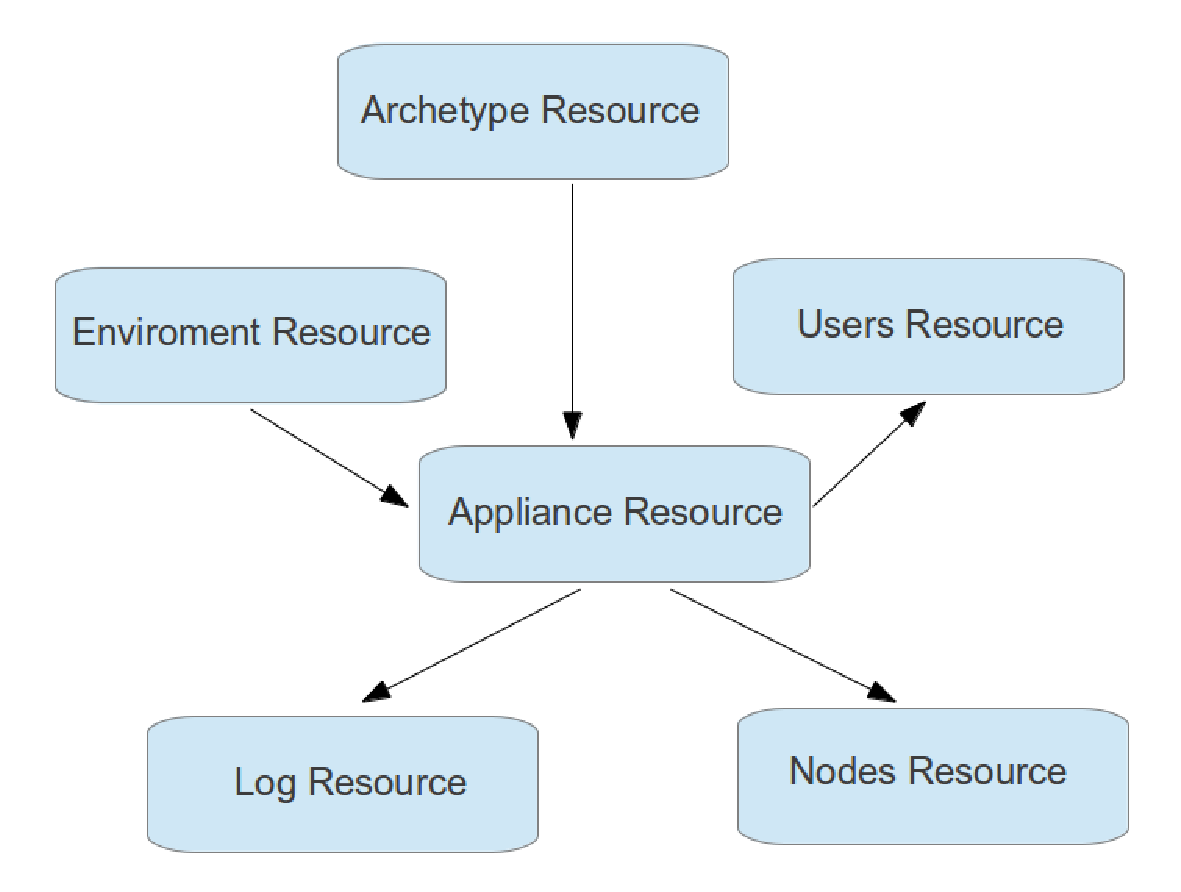
\includegraphics[scale=0.44]{fig/RelationshipsBetweenResources}
 \caption{Visi'on de las relaciones entre recursos}
 \label{fig:caption-bottom}
\end{figure}

El modelo de datos del Janu API esta basado en grupos de recursos, llamados colecciones:

\begin{description}
\item [Nodes collection] Un colecci'on de nodos consiste de todos los nodos que maneja el sistema. Es posible listar los nodos por pa'is o por ID.
\item [Log collection] Una colecci'on de logs consiste en todos los logs recibidos de los appliance. Es posible listar los logs por appliance, fecha o por tipo de log.
\item [Appliance collection] Una colecci'on de appliances consiste de todos los appliance registrados en el sistema. Es posible listarlos tambi'en por nodo o por ID.
\item [Enviroment collection] Una colecci'on de enviroments consiste de todas los enviroments creados en el sistema. Es posible listarlos por un usuario especifico.
\item [Archetype collection] Una colecci'on de arquetipos consiste en todos los arquetipos creados por los usuarios. Es posible listar los arquetipos por usuario, tipo o por ID.
\item [User collection] Una colecci'on de usuarios consiste en todos los usuarios con registrados en el sistema. Es posible listarlos por ID o por su propio identificador.
\end{description}

\section{Provisioning API reference}
El API esta organizado por tipo de recurso. Cada tipo de recurso tiene uno o mas representaciones de datos y uno o mas m'etodos.

Muchos recursos de este API retornan  <code>application/json</code> y esperan el http header <code>Accept: application/json</code>. Si se omite o falla en pasar este header en la petici'on http, la petici'on fallara.

\subsection{Nodes}

\begin{table}[h]
\scalebox{0.9}{
  \begin{tabular}{|l |l |p{9.3cm} |}
  \hline
  \rowcolor{blueapi}
    Method  & HTTP request & Description\\
    \hline
    list & GET /api/janu/nodes & Recibe una lista de recursos de nodos contenidos dentro del sistema.  \\
    \hline
    get & GET /api/janu/nodes/\{nodeId\} & Retorna el recurso de un nodo especifico.  \\
    \hline
    insert & POST /api/janu/nodes/\{nodeId\} & Crea un nuevo nodo en el sistema.  \\
    \hline
    update & PUT /api/janu/nodes/\{nodeId\} & Actualiza un nodo en el sistema.  \\
    \hline
    delete & DELETE /api/janu/nodes/\{nodeId\} & Elimina un nodo del sistema.  \\    
    \hline
  \end{tabular} 
  }
\caption[Nodes API]{Nodes API}
\label{tab:nodesapi}
\end{table}

\subsection{Log}

\begin{table}[h]
\scalebox{0.9}{
  \begin{tabular}{|l |l |p{8cm} |}
  \hline
  \rowcolor{blueapi}
    Method  & HTTP request & Description\\
    \hline
    list & GET /api/janu/log/node/\{nodeId\} & Recibe una lista de recursos de log de un nodo especifico.  \\
    \hline
    list & GET /api/janu/log/appliance/\{applianceId\} & Recibe una lista de recursos de log de un appliance especifico.  \\
    \hline
  \end{tabular} 
  }
\caption[Log API]{Log API}
\label{tab:logapi}
\end{table}

\newpage

\subsection{Appliance}

\begin{table}[h]
\scalebox{0.9}{
  \begin{tabular}{|l |p{9.7cm} |p{6cm} |}
  \hline
  \rowcolor{blueapi}
    Method  & HTTP request & Description\\
    \hline
    get & GET /api/janu/appliance/\{applianceId\} & Recibe un recurso de un appliance especifico.  \\
    \hline
    insert & POST /api/janu/appliance/\{applianceId\} & Crea un nuevo appliance en el sistema.  \\
    \hline
    update & PUT /api/janu/appliance/\{applianceId\} & Actualiza un appliance en el sistema.  \\
    \hline
    delete & DELETE /api/janu/appliance/\{applianceId\} & Elimina un appliance del sistema.  \\   
    \hline    
    stop & POST /api/janu/appliance/\{applianceId\}/stop & Detiene un appliance del sistema.  \\   
    \hline 
    start & POST /api/janu/appliance/\{applianceId\}/start & Inicia un appliance del sistema.  \\   
    \hline 
    clone & POST /api/janu/appliance/\{applianceId\}/clone & Clona un appliance del sistema.  \\   
    \hline    
    move & POST /api/janu/appliance/\{applianceId\}/move/node/ \{nodeId\} & Mueve un appliance a un nodo especifico.  \\   
    \hline   
    restart & POST /api/janu/appliance/\{applianceId\}/restart & Reinicia un appliance.  \\   
    \hline                 
  \end{tabular} 
  }
\caption[Appliance API]{Appliance API}
\label{tab:applianceapi}
\end{table}

\subsection{Enviroment}

\begin{table}[h]
\scalebox{0.9}{
  \begin{tabular}{|l |p{9.7cm} |p{6cm} |}
  \hline
  \rowcolor{blueapi}
    Method  & HTTP request & Description\\
    \hline
    get & GET /api/janu/enviroment/\{enviromentId\} & Recibe un recurso de un enviroment especifico.  \\
    \hline
    insert & POST /api/janu/enviroment/\{enviromentId\} & Crea un nuevo enviroment en el sistema.  \\
    \hline
    update & PUT /api/janu/enviroment/\{enviromentId\} & Actualiza un enviroment en el sistema.  \\
    \hline
    delete & DELETE /api/janu/enviroment/\{enviromentId\} & Elimina un enviroment del sistema.  \\   
    \hline    
  \end{tabular} 
  }
\caption[Enviroment API]{Enviroment API}
\label{tab:enviromentapi}
\end{table}

\subsection{Archetype}

\begin{table}[h]
\scalebox{0.9}{
  \begin{tabular}{|l |p{9.7cm} |p{6cm} |}
  \hline
  \rowcolor{blueapi}
    Method  & HTTP request & Description\\
    \hline
    get & GET /api/janu/archetype/\{archetypeId\} & Recibe un recurso de un archetype especifico.  \\
    \hline
    insert & POST /api/janu/archetype/\{archetypeId\} & Crea un nuevo archetype en el sistema.  \\
    \hline
    update & PUT /api/janu/archetype/\{archetypeId\} & Actualiza un archetype en el sistema.  \\
    \hline
    delete & DELETE /api/janu/archetype/\{archetypeId\} & Elimina un archetype del sistema.  \\   
    \hline    
  \end{tabular} 
  }
\caption[Archetype API]{Archetype API}
\label{tab:archetypeapi}
\end{table}

\newpage

\subsection{User}

\begin{table}[h]
\scalebox{0.9}{
  \begin{tabular}{|l |p{9.7cm} |p{6cm} |}
  \hline
  \rowcolor{blueapi}
    Method  & HTTP request & Description\\
    \hline
    list & GET /api/janu/user/ & Recibe una lista de recursos de usuarios del sistema.  \\    
    \hline
    get & GET /api/janu/user/\{userId\} & Recibe un recurso de un usuario especifico.  \\
    \hline
    insert & POST /api/janu/user/\{userId\} & Crea un nuevo usuario en el sistema.  \\
    \hline
    update & PUT /api/janu/user/\{userId\} & Actualiza un usuario en el sistema.  \\
    \hline
    delete & DELETE /api/janu/user/\{userId\} & Elimina un usuario del sistema.  \\   
    \hline    
  \end{tabular} 
  }
\caption[User API]{User API}
\label{tab:userapi}
\end{table}

\section{HTTP status codes}
La API de aprovisionamiento intenta devolver c'odigos de estado HTTP apropiados para cada solicitud. La siguiente tabla describe los c'odigo HTTP significativos en el contexto del API de aprovisionamiento.

\begin{table}[h]
\scalebox{0.9}{
  \begin{tabular}{|l |p{10.5cm}|}
  \hline
  \rowcolor{blueapi}
    Code  & Explanation \\
    \hline  
    200 Ok & No error. \\
    \hline
    201 Created & Creation of a resource was successful. \\
    \hline
    304 Not modified & The resource hasn't changed since the time specified in the request's If-Modified-Since header. \\
    \hline
    400 Bad request & Invalid request URI or header, or unsupported nonstandard parameter. \\
    \hline
    401 Unauthorized & Authorization required. \\
    \hline
    403 Forbidden & Unsupported standard parameter, or authentication or authorization failed. \\
    \hline
    404 Not found & Resource (such as a feed or entry) not found. \\
    \hline
    405 Method Not Allowed & The specified method is not allowed against this resource. \\
    \hline
    409 Conflict & Specified version number doesn't match resource's latest version number. \\
    \hline
    500 Internal server error & Internal error. This is the default code that is used for all unrecognized server errors. \\
    \hline   
    501 Not Implemented & A header you provided implies functionality that is not implemented. \\
    \hline
  \end{tabular} 
  }
\caption[HTTP status codes]{HTTP status codes}
\label{tab:httpstatuscodes}
\end{table}

\newpage

\section{El estilo REST}
REST es un estilo de arquitectura de software que proporciona un enfoque pr'actico y consistente para solicitar y modificar datos.

El termino REST es la abreviatura para \"Representational State Transfer.\" En el contexto del Janu API, se refiere al uso de verbos HTTP para recibir y modificar representaciones de datos guardadas por el sistema de aprovisionamiento.

En un sistema RESTful, los recursos se almacenan en un almac'en de datos, un usuario env'ia una solicitud al servidor para realizar una acci'on determinada (como la creaci'on, recuperaci'on, actualizaci'on o eliminaci'on de un recurso), y el servidor realiza la acci'on y env'ia una respuesta, a menudo en la forma de una representaci'on del recurso especificado.


En API REST de Janu, el usuario especifica una acci'on con un verbo HTTP como POST, GET, PUT o DELETE. Especifica un recurso por un URI 'unico global de la siguiente forma:

https://www.domain.edu.co/api/janu/resourcePath?parameters

Debido a que todos los recursos del API tienen 'unica URI HTTP accesible, REST permite el almacenamiento en cach'e de datos y est'a optimizado para trabajar con una infraestructura distribuida de la web.

\section{Formato de datos - JSON}
JSON (JavaScript Object Notation) es un formato de datos com'un, independiente del lenguaje que proporciona una representaci'on de texto simple de estructuras de datos arbitrarias. Para obtener m'as informaci'on, ver json.org.

\section{Ejemplos}


\section{Autenticaci'on}

La autenticaci'on es el proceso de demostrar la identidad al sistema. La identidad es un factor importante en las decisiones de control de acceso. Las solicitudes se conceden o deniegan en parte sobre la base de la identidad del solicitante.

El Janu API REST utiliza un esquema HTTP personalizado basado en una llave-HMAC (Hash Message Authentication Code) para la autenticaci'on.Para autenticar una solicitud, primero se concatenan los elementos seleccionados de la solicitud para formar una cadena. A continuaci'on, utiliza una clave secreta de acceso para calcular el HMAC de esa cadena. Informalmente, llamamos a este proceso \"la firma de la solicitud\", y llamamos a la salida del algoritmo HMAC la \"firma\", ya que simula las propiedades de seguridad de una firma real. Por 'ultimo, se agrega esta firma como un par'ametro de la petici'on, con la sintaxis descrita en esta secci'on.

Cuando el sistema recibe una solicitud fehaciente, se obtiene la clave secreta de acceso que dicen tener, y lo utiliza de la misma manera que se calcula una \"firma\" del mensaje que recibi'o. A continuaci'on, compara la firma que se calcula con la firma presentada por el solicitante. Si las dos firmas coinciden, el sistema llega a la conclusi'on de que el solicitante debe tener acceso a la clave secreta de acceso, y por lo tanto act'ua con la autoridad del principal al que se emiti'o la clave. Si las dos firmas no coinciden, la solicitud se descarta y el sistema responde con un mensaje de error.

Ejemplo de una petici'on autenticada:

\medskip
\begin{lstlisting}
  GET /api/janu/appliance/{applianceId} HTTP/1.1
  Host: host1.edu.co
  Date: Fri, 01 Jul 2011 19:37:58 +0000

  Authorization: 0PN5J17HBGZHT7JJ3X82:frJIUN8DYpKDtOLCwo//yllqDzg= 
\end{lstlisting}

\subsection{Authentication Header}

El API REST utiliza el encabezado de autorizaci'on HTTP est'andar para pasar informaci'on de autenticaci'on. (El nombre de la cabecera est'andar es insuficiente, ya que solo lleva la informaci'on de autenticaci'on y no la de autorizaci'on). Bajo el esquema de autenticaci'on de Janu, el encabezado de autorizaci'on tiene la siguiente forma.

\medskip
\begin{lstlisting}
  Authorization: JanuUserId:Signature
\end{lstlisting}

Los usuarios tendr'an un ID de clave de acceso (Janu Access Key ID) y una clave secreta de acceso (Janu Secret Access Key) cuando se registran. Para la petici'on de autenticaci'on, el elemento de Janu Access Key Id identifica la clave secreta que se utiliz'o para calcular la firma, y (indirectamente) el usuario que realiza la solicitud.

Para la firma de los elementos de la petici'on se usa el RFC 2104HMAC-SHA1, por lo que la parte de la firma de la cabecera autorizaci'on variar'a de una petici'on a otra. Si la solicitud de la firma calculada por el sistema coincide con la firma incluida en la solicitud, el solicitante habr'a demostrado la posesi'on de la clave secreta de acceso. La solicitud ser'a procesada bajo la identidad, y con la autoridad, de la promotora que se emiti'o la clave.

A continuaci'on se muestra la pseudo-gramática que ilustra la construcci'on de la cabecera de la solicitud de autorizaci'on (
\textbackslash{}n significa el punto de c'odigo Unicode U +000 A com'unmente llamado salto de l'inea).

\medskip
\begin{lstlisting}
  Authorization = JanuUserId + ":" + Signature;

  Signature = Base64( HMAC-SHA1( UTF-8-Encoding-Of( YourSecretAccessKeyID, StringToSign ) ) );

  StringToSign = HTTP-Verb + "\n" +
  Host + "\n" +
  Content-MD5 + "\n" +
  Content-Type + "\n" +
  Date + "\n" +
  CanonicalizedResource;

  CanonicalizedResource = <HTTP-Request-URI, from the protocol name up to the query string (resource path)>
\end{lstlisting}

HMAC-SHA1 es un algoritmo definido por la RFC 2104 (ver la RFC 2104 con llave Hashing para la autenticaci'on de mensajes).
El algoritmo toma como entrada dos cadenas de bytes: una clave y un mensaje. Para la solicitud de autenticaci'on, se utiliza la clave secreta (YourSecretAccessKeyID) como la clave, y la codificaci'on UTF-8 del StringToSign como el mensaje. La salida de HMAC-SHA1 es tambi'en una cadena de bytes, llamado el resumen. El par'ametro de la petici'on de la Firma se construye codificada en Base64.

\subsection{Solicitud can'onica para firmar}

Cuando el sistema recibe una solicitud autenticada, compara la solicitud de firma calculada con la firma proporcionada en la solicitud de StringToSign. Por esta raz'on, se debe calcular la firma con el mismo m'etodo utilizado por Janu. A este proceso de poner una solicitud en una forma acordada para la firma se denomino "canonizaci'on".

\subsection{Tiempo de sello}

Un sello de tiempo v'alido (utilizando el HTTP header Date) es obligatorio para solicitudes autenticadas. Por otra parte, el tiempo del sello enviado por un usuario que se encuentra incluido en una solicitud autenticada debe estar dentro de los 15 minutos de la hora del sistema cuando se recibe la solicitud. En caso contrario, la solicitud fallar'a con el c'odigo de estado de error RequestTimeTooSkewed. La intenci'on de estas restricciones es limitar la posibilidad de que solicitudes interceptadas pueden ser reproducidos por un adversario.Para una mayor protecci'on contra las escuchas, se debe utilizar el transporte HTTPS para solicitudes autenticadas.

\subsection{Ejemplos de autenticaci'on}

\begin{tabular}{|l|l|} \hline
\textbf{Parametro} & \textbf{Valor} \\ \hline
JanuUserId  & 13010f3e-3f46-4889-b989-592ce8fb30c6 \\ \hline
\multicolumn{1}{|m{3.7cm}|}{
JanuSecretAccessKey} & \multicolumn{1}{m{12.5cm}|}%
{\raggedright c991f519-bed0-4dab-9165-6d9f722dc845 \\
\textbf{Base64:} \\ Yzk5MWY1MTktYmVkMC00ZGFiLTkxNjUtNmQ5ZjcyMmRjODQ1} \tabularnewline \hline
\end{tabular}

\textbf{Ejemplo de un objeto con GET}

Este es un ejemplo que consulta por un enviroment dado su identificador.

\begin{tabular}{|l|l|} \hline
\textbf{Request} & \textbf{StringToSign} \\ \hline
\multicolumn{1}{|m{10.5cm}|}%
{\raggedright GET /api/janu/enviroment/45 HTTP/1.1 \\
 Host: host1.edu.co \\
 Date: Tue, 27 Mar 2007 19:36:42 +0000 \\
 Authorization: 13010f3e-3f46-4889-b989-592ce8fb30c6: Yzk5MWY1MmVkMC00ZGFiLTtNmQ5ZjcyMmRjODQ1 } & \multicolumn{1}{m{6.5cm}|}%
{\raggedright GET\textbackslash{}n \\
 host1.edu.co\textbackslash{}n \\
 \textbackslash{}n \\
 \textbackslash{}n \\
 Tue, 27 Mar 2007 19:36:42 +0000\textbackslash{}n \\ /api/janu/enviroment/45} \tabularnewline \hline
\end{tabular}

\textbf{Ejemplo de un objeto con DELETE}

Este ejemplo remueve un usuario.

\begin{tabular}{|l|l|} \hline
\textbf{Request} & \textbf{StringToSign} \\ \hline
\multicolumn{1}{|m{10.5cm}|}%
{\raggedright DELETE /api/janu/user/9876 HTTP/1.1 \\
 Host: host1.edu.co \\
 Date: Tue, 27 Mar 2007 21:20:27 +0000 \\
 Authorization: 13010f3e-3f46-4889-b989-592ce8fb30c6: Yzk5MWY1MmVkMC00ZGFiLTtNmQ5ZjcyMmRjODQ1 } & \multicolumn{1}{m{6.5cm}|}%
{\raggedright DELETE\textbackslash{}n \\
 host1.edu.co\textbackslash{}n \\
 \textbackslash{}n \\
 \textbackslash{}n \\
 Tue, 27 Mar 2007 21:20:27 +0000\textbackslash{}n \\ /api/janu/user/9876} \tabularnewline \hline
\end{tabular}






